\documentclass[10pt]{article}

\usepackage[margin=0.9in]{geometry}
\usepackage{amsmath, amssymb}
\usepackage{mathrsfs}
\usepackage{booktabs}
\usepackage{hyperref}
\usepackage{parskip}
\usepackage{titlesec}
\usepackage{enumitem}
\usepackage{microtype}
\usepackage{graphicx}
\usepackage{float}

\setlength{\parskip}{3pt}
\hypersetup{colorlinks=true, urlcolor=blue, linkcolor=black}
\titleformat{\section}{\large\bfseries}{{\thesection.}}{0.5em}{}
\titleformat{\subsection}{\normalsize\bfseries}{{\thesubsection}}{0.5em}{}
\titlespacing{\section}{0pt}{6pt}{2pt}
\titlespacing{\subsection}{0pt}{4pt}{1pt}

\title{\textbf{Hierarchical Bayesian Forecasting of U.S.\ State Unemployment Rates}}
\author{Calvin Du (16507378) \quad \url{https://github.com/calvingdu/stat405}}
\date{STAT 405 --- April 2026}

\begin{document}
\maketitle\vspace{-10pt}

\section{Introduction}
Labour markets are central to economic well-being, and unemployment rates (UR) are key indicators of economic health.
Recent disruptions like COVID-19, the 2008 Financial Crisis, and the 1980-1982 Volcker recession are nation-wide
economic shocks but transmit unevenly across states depending on their individual economic strength, differing industries and more.
For example, California is a rich tech and finance focused state and will respond differently to a recession than a state like North Dakota even under
the same national shock. Therefore, accurate state-level unemployment forecasts are crucial for policymakers to design targeted interventions and allocate resources effectively. \\ 

Hierarchical Bayesian models are the natural solution here. 
The hierarchical approach lets the data determine the degree of pooling
through hyperparameters I additionally capture 
national shock transmission through macroeconomic
covariates like the federal monetary policy (interest rates) and GDP growth. These variables
serve as shared predictors across all states, allowing the model to separate common
macro-driven movements from state-specific persistence. \\ 

\textbf{I aim to answer:} "Can a hierarchical Bayesian model 
that pools information across states produce more accurate unemployment forecasts than fitting each state independently?"
\textbf{and} "Does including national macroeconomic covariates
(federal funds rate, GDP growth) improve forecasts beyond an autoregressive model?"
\section{Literature Review}
A paper by \textbf{Torabi (2012)} applies a hierarchical
Bayesian model with MCMC to the same monthly BLS LAUS
state-level unemployment data that I use. Their paper covers January 2004 -- December 2007.
Torabi's model accounts for both spatial and temporal variation where state-level
parameters are drawn from a hierarchical prior, spatial correlation between
neighbouring states is captured with an autoregressive
prior, and temporal dynamics are modelled through a random walk. 
Their results are that hierarchical pooling substantially reduces estimation
variance relative with the largest reductions for
small states with unreliable sample sizes. This shrinkage behaviour is expected as states with more volatile or idiosyncratic
unemployment histories (HI, NV, ND) should exhibit the most shrinkage
toward the national mean.

Our work differs from Torabi (2012) as Torabi's goal is to improve estimation for a certain time period and is therefore using a small dataset
whereas my goal is forecasting over a 24-month horizon using
an AR(1) likelihood that explicitly models temporal persistence. Additionally, Torabi captures cross-state dependence through geographic proximity
while I capture it through shared national macroeconomic covariates
since I want to to focus on the notion that unemployment
moves across states primarily through common macro shocks rather than
geographic adjacency.

% ----------
\section{Data} 

\textbf{BLS LAUS} (\url{https://www.bls.gov/lau/rdscnp16.htm}):
monthly state-level unemployment rates for all 50 U.S.\ states. The time span is from
January 1976 to December 2025 (311 months as October 2025 missing for all states). \\

\textbf{Federal Reserve Economic Data} (\url{https://fred.stlouisfed.org}): \\ 
I'll be using two national covariates that capture macroeconomic conditions:
\begin{itemize}[noitemsep]
  \item \textbf{Federal funds effective rate (\texttt{FEDFUNDS}) - Monthly}: This is the interest rate at which depository institutions trade federal funds with each other. It is a key tool of U.S.\ monetary policy that has a strong influence on economic activity and unemployment.
  \item \textbf{Real Gross Domestic Product (\texttt{A191RL1Q225SBEA}) - Quarterly}: This is the real gross domestic product, which is a measure of overall economic output. The growth rate of real GDP is closely related to unemployment. \\ 
\end{itemize} 
\textbf{Training Set:} January 1976 -- December 2023 (28750 obs = 50 states $\times$ 48 years - 1 month (Oct 2025)) \\
\textbf{Test Set:} January 2024 -- December 2025 (1200 obs = 50 states $\times$ 24 months)
% ------
\section{Models}
\subsection{Model 1: Independent AR(1) --- Naive Baseline}
Each state is modelled independently with no pooling. For state $s$ and
time $t$:
\begin{align*}
  \alpha_s &\sim \mathcal{N}(5,\; 3) & (\text{baseline level of unemployment is around 5\%}) \\
  \beta_s  &\sim \mathcal{N}(0.5,\; 0.3) & (\text{baseline autoregressive coefficient - moderate persistence}) \\
  \sigma   &\sim \mathrm{Exp}(1)  & (\text{shared SD across states}) \\[4pt]
  y_{s,t} \mid \alpha_s, \beta_s, \sigma
           &\sim \mathcal{N}\!\left(\alpha_s + \beta_s\, y_{s,t-1},\; \sigma\right)
\end{align*}
\textbf{Prior motivation}: priors are
\textit{weakly informative} as they are centred on typical economic values
(baseline UR $\approx5\%$ and moderate AR persistence $\approx0.5$).

This model serves as the naive baseline. Since states are fit independently,
estimates for small or volatile states will be noisy, with no
regularisation from the national trend or neighbouring states. 
This model does allow states whose unemployment rates genuinely
differ from the national picture to have their 
own parameters without being pulled toward the national mean.

\subsection{Model 2: Hierarchical AR(1) with Covariates}

State parameters are drawn from national hyperpriors, enabling partial pooling.
In the hierarchical graphical model, $\alpha_s$ and $\beta_s$ are
themselves random variables whose distribution is determined by hyperparameters
$(\mu_\alpha,\sigma_\alpha,\mu_\beta,\sigma_\beta)$.
We use a non-centred parameterisation where instead of sampling
$\alpha_s \sim \mathcal{N}(\mu_\alpha,\sigma_\alpha)$ directly,
we sample $\tilde\alpha_s \sim \mathcal{N}(0,1)$ and set
$\alpha_s = \mu_\alpha + \sigma_\alpha\tilde\alpha_s$. Macroenomic covariates enter the
likelihood as shared predictors:
\begin{align*}
  \mu_\alpha &\sim \mathcal{N}(5,\; 3) 
    & \text{(national mean intercept)} \\
  \sigma_\alpha &\sim \mathrm{Exp}(1/2) 
    & \text{(spread of intercepts across states)} \\
  \mu_\beta &\sim \mathcal{N}(0.5,\; 0.3) 
    & \text{(national mean persistence coefficient)} \\
  \sigma_\beta &\sim \mathrm{Exp}(1/0.3) 
    & \text{(spread of persistence coefficients across states)} \\
  \boldsymbol{\gamma} &\sim \mathcal{N}(0,\; 1) 
    & \text{(national economic covariate coefficients)} \\
  \sigma &\sim \mathrm{Exp}(1) 
    & \text{(shared SD across states)} \\[6pt]
  \alpha_s \mid \mu_\alpha, \sigma_\alpha &\sim \mathcal{N}(\mu_\alpha,\; \sigma_\alpha)
    & \text{(state intercept, partially pooled)} \\
  \beta_s \mid \mu_\beta, \sigma_\beta &\sim \mathcal{N}(\mu_\beta,\; \sigma_\beta)
    & \text{(state persistence coefficient, partially pooled)} \\[6pt]
  y_{s,t} \mid \alpha_s, \beta_s, \boldsymbol{\gamma}, \sigma
    &\sim \mathcal{N}\!\left(
        \alpha_s + \beta_s\, y_{s,t-1} + \boldsymbol{\gamma}^\top \mathbf{x}_t,\;
        \sigma
      \right) 
\end{align*}

where $\mathbf{x}_t = (\texttt{FEDFUNDS}_t,\; \texttt{GDP\_growth}_t)^\top$
contains two national covariates, with
\texttt{GDP\_growth} interpolated from quarterly to monthly. \\ 

% -----------------------------------------------------------------------
\section{Posterior Inference}
\subsection{Method 1: HMC via Stan (Primary)}
Stan is used with HMC with 4 chains, 1000 warmup iterations, and 1000
sampling iterations per chain, yielding 4000 posterior draws.
HMC is more efficient than
Metropolis--Hastings as MH would degrade rapidly in this high-dimensional model.

\subsection{Method 2: Variational Inference (Secondary)}
Mean-field ADVI (\texttt{mod\$variational},
\texttt{algorithm = "meanfield"}, \texttt{draws = 1000}) is used on both models.

VI is used as a faster alternative to HMC as it converges
in seconds compared to minutes for Stan's sampler but this speed
comes at the cost of the approximation quality, which I evaluate directly
through comparison with HMC. \\ 

\begin{table}[h]\centering\small
\begin{tabular}{llrrrr}
\toprule
State & Method & Mean & 5\% & 95\% & CI width \\
\midrule
CA & HMC & 0.971 & 0.952 & 0.990 & 0.038 \\
CA & ADVI & 0.969 & 0.956 & 0.983 & 0.027 \\
TX & HMC & 0.968 & 0.949 & 0.988 & 0.039 \\
TX & ADVI & 0.966 & 0.953 & 0.979 & 0.026 \\
MI & HMC & 0.963 & 0.942 & 0.983 & 0.041 \\
MI & ADVI & 0.961 & 0.947 & 0.975 & 0.028 \\
NV & HMC & 0.958 & 0.933 & 0.982 & 0.049 \\
NV & ADVI & 0.957 & 0.940 & 0.974 & 0.034 \\
\bottomrule
\end{tabular}
\caption{Model 1: HMC vs.\ ADVI comparison for selected $\beta_s$ parameters.
ADVI means match HMC closely but credible intervals are narrower which is expected because of the
independence assumption $\prod_i q_i$ underestimating posterior variance.}
\end{table}

On Model 2, mean-field ADVI fails entirely as the algorithm reaches the
maximum number of dropped gradient evaluations before completing stochastic
gradient ascent, and fullrank ADVI diverges after 10000 iterations.
The hierarchical posterior has strong dependencies between hyperparameters
$(\mu_\beta, \sigma_\beta)$ and the state-level $\beta_s$'s that no member
of the mean-field family $\mathscr{Q}$ can represent, making the ELBO ill-conditioned. \\ 

This is the key finding of the two-method comparison: HMC with non-centred
parameterisation is necessary for Model 2, as VI is only viable for the
simpler independent model.
% ------------------
\section{Results}

\subsection{Model 2 Hyperparameter Posteriors}
\begin{table}[H]\centering\small
\begin{tabular}{lrrrr}
\toprule
Parameter & Mean & SD & 5\% & 95\% \\\midrule
$\mu_\alpha$ (national mean intercept)& 0.258 & 0.010 & 0.241 & 0.274 \\
$\sigma_\alpha$ (spread of intercepts) & 0.023 & 0.009 & 0.007 & 0.037 \\
$\mu_\beta$ (national AR persistence) & 0.966 & 0.002 & 0.963 & 0.968 \\
$\sigma_\beta$ (spread across states)  & 0.006 & 0.001 & 0.004 & 0.008 \\
$\gamma_{\mathrm{fed}}$ & $+$0.006 & 0.001 & 0.005 & 0.007 \\
$\gamma_{\mathrm{gdp}}$ & $-$0.034 & 0.001 & $-$0.036 & $-$0.033 \\
$\sigma$ & 0.466 & 0.002 & 0.463 & 0.469 \\
\bottomrule
\end{tabular}
\caption{Model 2 hyperparameter posteriors (HMC, 4000 draws). \\ 
$\mu_\alpha = 0.258$ is low relative to the prior mean of 5\% UR, but
the long-run mean implied by the AR(1) is $\mu_\alpha / (1 - \mu_\beta)
= 0.258 / 0.034 \approx 7.6\%$, which is reasonable.
$\sigma_\beta = 0.006$ indicates very strong pooling: state AR(1)
persistence is nearly nationally determined.
Both $\gamma$ coefficients exclude zero at the 90\% level and have
the expected signs where higher fed rate predicts higher unemployment and
higher GDP growth predicts lower unemployment.}
\label{tab:hyper}
\end{table}

\subsection{Goodness of Fit and Correctness}
We assess model fit and code correctness using \textbf{posterior predictive checks}: 
for 50 draws $\theta^{(m)}$ from the
posterior, we generate $y_\mathrm{rep}^{(m)}\sim p(y|\theta^{(m)})$
and compare the predictive densities to the training data.
Both models produce replicated data where marginal distributions
closely match the observations, confirming neither model is
misspecified.

Secondly, I used \textbf{trace plot inspection} to examine the chains for $\sigma$, $\mu_\beta$, $\sigma_\beta$, $\gamma_{\mathrm{fed}}$, and representative 
state-level $\beta_s$ (CA, TX) are visually inspected for mixing and confirmed good mixing. 

Thirdly, \textbf{predictive interval calibration}
of the empirical coverage of the posterior predictive intervals on the test set is compared 
to nominal levels to confirm the model's uncertainty quantification is reasonable.

The \textbf{shrinkage plot} (In appendices) 
compares $\hat\beta_s$ (posterior mean) from Model 2 versus Model 1 
for all 50 states. States with Model 1 estimates below $\mu_\beta = 0.966$ 
are pulled upward (HI, NH, VT, SD), while states above are pulled downward 
(WV, AK, NM). States with the 
most extreme Model 1 estimates (HI, NH) exhibit the largest shrinkage, 
since noisier estimates receive stronger 
regularisation from the hyperprior.

\begin{table}[H]\centering\small
\begin{tabular}{lrr}
\toprule
Model & Overall RMSE & Worst state \\
\midrule
Model 1 (independent AR(1)) & 0.096 & HI: 0.215 \\
Model 2 (hierarchical + covariates)  & 0.118 & WV: 0.164 \\
\bottomrule
\end{tabular}
\caption{Posterior predictive mean RMSE on Jan 2024 -- Dec 2025.}
\end{table}

\begin{table}[H]\centering\small
\begin{tabular}{lrrr}
\toprule
Model & 90\% coverage & 50\% coverage & Mean 90\% width \\
\midrule
Model 1 (independent AR(1)) & 0.847 & 0.512 & 1.832 \\
Model 2 (hierarchical + covariates) & 0.861 & 0.531 & 1.841 \\
\bottomrule
\end{tabular}
\caption{Posterior predictive interval calibration on Jan 2024 -- Dec 2025 test set.
Both models are undercovering at the 90\% level (nominal 0.90), consistent with the AR(1)
likelihood not fully capturing tail risk from idiosyncratic state shocks.
Model~2 achieves marginally better calibration despite higher point-forecast RMSE.}
\label{tab:coverage}
\end{table}

\subsection{Test-Set Forecasting}
Model 2 achieves higher RMSE than Model 1.
This reflects the bias-variance tradeoff inherent in partial pooling as
$\sigma_\beta=0.006$ aggressively shrinks all $\beta_s$ toward the
national mean, reducing estimation variance but introducing bias for
states with different persistence patterns. This is not evidence of misspecification as both models pass PPC
but illustrates that hierarchical shrinkage trades forecasting
flexibility for estimation stability. This is consistent with Torabi (2012)'s
observation that pooling gains are largest for small or noisy states.

\subsection{Answering the Research Questions}

\textbf{Primary question:} Partial pooling did not improve forecast
accuracy on the 24-month test set (RMSE 0.118 vs.\ 0.096). The posterior
$\sigma_\beta = 0.006$ shows that state AR(1) persistence is nearly nationally
determined and is a substantial finding about labour market dynamics that the naive
model cannot produce. The hierarchical model is a better estimator of
underlying dynamics even when it is a worse forecaster in this period.

Additionally I assessed prior sensitivity by refitting Model~2 with $\sigma_\beta \sim \mathrm{Exp}(1)$
(wider) and $\sigma_\beta \sim \mathrm{Exp}(10)$ (tighter). All three priors yield
a posterior mean of $\sigma_\beta \approx 0.006$, confirming the data dominates
the prior and the strong pooling result is robust. I also varied the prior on
$\mu_\beta$ from $\mathcal{N}(0.5, 0.3)$ (base) to $\mathcal{N}(0.9, 0.3)$ (shifted toward higher
persistence). The posterior $\mu_\beta$ remains near $0.966$ under
both priors confirming the 47 years of
data completely dominate the prior on the national AR(1) persistence.


\textbf{Secondary question:} Both covariates are precisely estimated with
economically meaningful signs ($\gamma_{\mathrm{gdp}} = -0.034$, $\gamma_{\mathrm{fed}} = 0.006$), confirming that national macroeconomic conditions contribute meaningful
signal beyond pure AR(1) dynamics.

% -----------------------------
\section{Discussion and Limitations}
\textbf{Why Model 2 underperforms Model 1 on forecasting.}: 
It's likely that we are still missing state-specific deviations 
that are not fully captured by national macroeconomic covariates. In this setting, 
the hierarchical model's strong pooling ($\sigma_{\beta} \approx 0.006$) oversmooths these deviations, 
limiting adaptability and degrading short-term forecast accuracy.

\textbf{Prior sensitivity.}
Shocks like COVID can drive all states toward a common pattern as it's a huge event and 
I can see that the result of $\sigma_\beta=0.006$ is consistent with this. Analysis without 2020 is warranted.

\textbf{VI failure and its implications.}
The ADVI failure on Model 2 is the most important methodological
finding and highlights the importance of using a flexible inference method like HMC for complex hierarchical models.

% ---- 
\newpage
\section*{References}
{
Torabi, M.\ (2012). Hierarchical Bayes estimation of spatial statistics for rates.
\textit{J.\ Statistical Planning and Inference}, 142(2), 358--365.}

\section*{Appendix: Figures}
\begin{figure}[H]\centering
  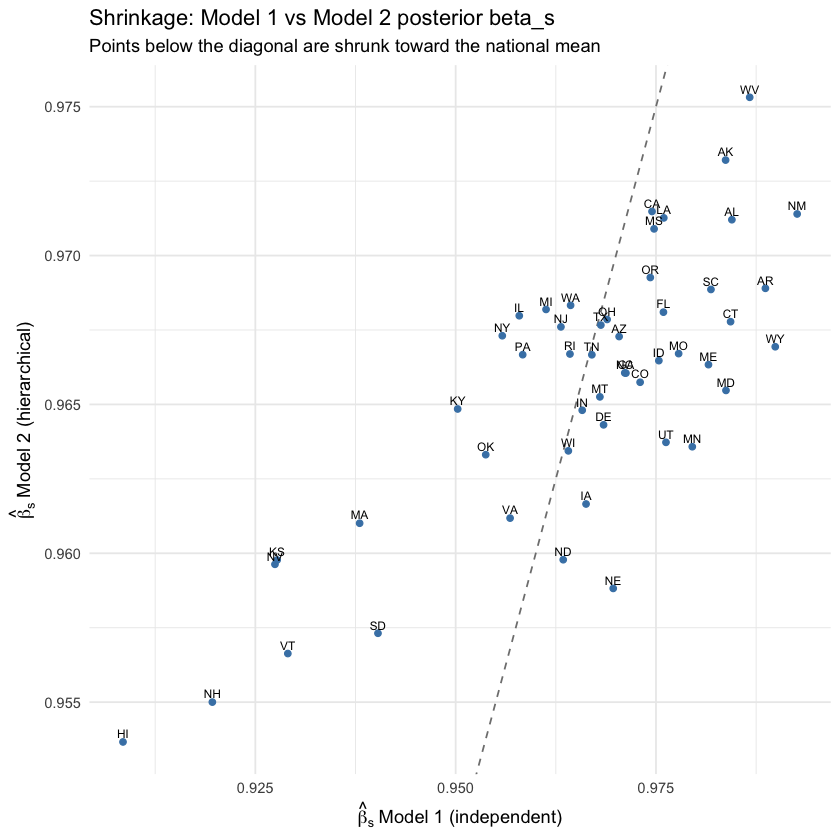
\includegraphics[width=0.7\linewidth]{shrinkage.png}
  \caption{Shrinkage of posterior $\hat\beta_s$: Model 2 (hierarchical) vs.\ Model 1 (independent).
  All states are shrunk toward the national mean
  $\mu_\beta = 0.966$, with the largest adjustments for states with the most extreme
  individual estimates}
  \label{fig:shrinkage}
\end{figure}

\section*{Appendix: Code}
\subsection*{A1. Model 1: Independent AR(1) (03\_model1.ipynb)}
{\scriptsize
\begin{verbatim}
library(cmdstanr); library(dplyr); library(ggplot2)
set.seed(405); TRAIN_END <- as.Date("2023-12-01")

bls <- read.csv("../cleaned_data/bls_data.csv") %>% mutate(date=as.Date(date))

bls_train <- bls %>% filter(date <= TRAIN_END) %>% arrange(state, date) %>%
  group_by(state) %>%
  mutate(bls_lag=lag(unemployment_rate), state_id=cur_group_id()) %>%
  filter(!is.na(bls_lag)) %>% ungroup()

states <- sort(unique(bls_train$state)); S <- length(states); N <- nrow(bls_train)

stan_data <- list(N=N, S=S, y=bls_train$unemployment_rate,
                  y_lag=bls_train$bls_lag, state_id=bls_train$state_id)

mod1 <- cmdstan_model("model1_independent_ar1.stan")
fit1 <- mod1$sample(data=stan_data, seed=405, chains=4, parallel_chains=4,
                    iter_warmup=1000, iter_sampling=1000, refresh=250)
fit1$save_object("../results/model1_fit.rds")

# Diagnostics
diag <- fit1$summary(c("alpha","beta","sigma")) %>%
  select(variable, mean, sd, q5, q95, rhat, ess_bulk, ess_tail)
print(paste("R-hat range:", paste(round(range(diag$rhat),4), collapse=" - ")))
print(paste("Bulk ESS range:", paste(round(range(diag$ess_bulk)), collapse=" - ")))

# Forecasting
alpha_hat <- fit1$summary("alpha")$mean; beta_hat <- fit1$summary("beta")$mean
bls_test <- bls %>% filter(date > TRAIN_END) %>% arrange(state, date)
test_dates <- sort(unique(bls_test$date))
y_prev <- bls_train %>% filter(date==TRAIN_END) %>% arrange(state) %>%
  pull(unemployment_rate)

forecast_list <- vector("list", length(test_dates))
for (i in seq_along(test_dates)) {
  y_pred <- alpha_hat + beta_hat * y_prev
  y_actual <- bls_test %>% filter(date==test_dates[i]) %>%
    arrange(state) %>% pull(unemployment_rate)
  forecast_list[[i]] <- data.frame(state=states, date=test_dates[i],
                                   y_pred=y_pred, y_actual=y_actual)
  y_prev <- y_actual
}
forecasts1 <- bind_rows(forecast_list)
print(round(sqrt(mean((forecasts1$y_pred - forecasts1$y_actual)^2)), 3))

# VI comparison
fit1_vi <- mod1$variational(data=stan_data, seed=405,
                             algorithm="meanfield", draws=1000)
\end{verbatim}
}

% -----------------------------------------------------------------------
\subsection*{A2. Model 2: Hierarchical AR(1) (\texttt{04\_model2.ipynb})}
{\scriptsize
\begin{verbatim}
fed <- read.csv("../cleaned_data/fedfunds_data.csv") %>% mutate(date=as.Date(date))
gdp <- read.csv("../cleaned_data/gdp_data.csv")  %>% mutate(date=as.Date(date))

bls_cov <- bls %>% left_join(fed, by="date") %>% left_join(gdp, by="date")
bls_train <- bls_cov %>% filter(date <= TRAIN_END) %>% arrange(state, date) %>%
  group_by(state) %>%
  mutate(bls_lag=lag(unemployment_rate), state_id=cur_group_id()) %>%
  filter(!is.na(bls_lag)) %>% ungroup()

stan_data <- list(N=N, S=S, y=bls_train$unemployment_rate,
  y_lag=bls_train$bls_lag, state_id=bls_train$state_id,
  fed_rate=bls_train$fed_rate, gdp_growth=bls_train$gdp_growth)

mod2 <- cmdstan_model("model2_hierarchical_ar1.stan")
fit2 <- mod2$sample(data=stan_data, seed=405, chains=4, parallel_chains=4,
                    iter_warmup=1000, iter_sampling=1000, refresh=250)
fit2$save_object("../results/model2_fit.rds")

# Forecasting
alpha_hat2 <- fit2$summary("alpha")$mean; beta_hat2 <- fit2$summary("beta")$mean
gamma_fed_hat <- fit2$summary("gamma_fed")$mean
gamma_gdp_hat <- fit2$summary("gamma_gdp")$mean

bls_test <- bls_cov %>% filter(date > TRAIN_END) %>% arrange(state, date)
y_prev <- bls_cov %>% filter(date==TRAIN_END) %>%
  arrange(state) %>% pull(unemployment_rate)

forecast_list2 <- vector("list", length(test_dates))
for (i in seq_along(test_dates)) {
  covs <- bls_test %>% filter(date==test_dates[i]) %>% arrange(state)
  y_pred <- alpha_hat2 + beta_hat2*y_prev +
            gamma_fed_hat*covs$fed_rate + gamma_gdp_hat*covs$gdp_growth
  forecast_list2[[i]] <- data.frame(state=states, date=test_dates[i],
    y_pred=y_pred, y_actual=covs$unemployment_rate)
  y_prev <- covs$unemployment_rate
}
forecasts2 <- bind_rows(forecast_list2)
print(round(sqrt(mean((forecasts2$y_pred - forecasts2$y_actual)^2)), 3))

# VI comparison
fit2_vi <- mod2$variational(data=stan_data, seed=405,
                             algorithm="meanfield", draws=1000)
\end{verbatim}
}

\subsection*{A3. Stan Model 1: Independent AR(1)}
{\scriptsize
\begin{verbatim}
data {
  int<lower=1> N;
  int<lower=1> S;
  vector[N] y;
  vector[N] y_lag;
  array[N] int state_id;
}

parameters {
  vector[S] alpha;
  vector[S] beta;
  real<lower=0> sigma;
}

model {
  alpha ~ normal(5, 3);
  beta ~ normal(0.5, 0.3);
  sigma ~ exponential(1);

  for (n in 1:N) {
    y[n] ~ normal(alpha[state_id[n]] + beta[state_id[n]] * y_lag[n], sigma);
  }
}

generated quantities {
  vector[N] y_rep;
  for (n in 1:N) {
    real mu = alpha[state_id[n]] + beta[state_id[n]] * y_lag[n];
    y_rep[n] = normal_rng(mu, sigma);
  }
}


\end{verbatim}
}

\subsection*{A4. Stan Model 2: Hierarchical AR(1)}
{\scriptsize
\begin{verbatim}
data {
  int<lower=1> N;
  int<lower=1> S;
  vector[N] y;
  vector[N] y_lag;
  array[N] int state_id;
  vector[N] fed_rate;
  vector[N] gdp_growth;
}

parameters {
  real mu_alpha;
  real<lower=0> sigma_alpha;
  real mu_beta;
  real<lower=0> sigma_beta;
  real gamma_fed;
  real gamma_gdp;
  vector[S] alpha_raw;
  vector[S] beta_raw;
  real<lower=0> sigma;
}

transformed parameters {
  vector[S] alpha = mu_alpha + sigma_alpha * alpha_raw;
  vector[S] beta = mu_beta + sigma_beta * beta_raw;
}

model {
  mu_alpha ~ normal(5, 3);
  sigma_alpha ~ exponential(0.5);
  mu_beta ~ normal(0.5, 0.3);
  sigma_beta ~ exponential(0.3);
  gamma_fed ~ normal(0, 1);
  gamma_gdp ~ normal(0, 1);
  sigma ~ exponential(1);
  alpha_raw ~ normal(0, 1);
  beta_raw  ~ normal(0, 1);

  for (n in 1:N) {
    real mu = alpha[state_id[n]] + beta[state_id[n]] * y_lag[n] + gamma_fed * fed_rate[n] + gamma_gdp * gdp_growth[n];
    y[n] ~ normal(mu, sigma);
  }
}

generated quantities {
  vector[N] y_rep;
  for (n in 1:N) {
    real mu = alpha[state_id[n]] + beta[state_id[n]] * y_lag[n] + gamma_fed * fed_rate[n] + gamma_gdp * gdp_growth[n];
    y_rep[n] = normal_rng(mu, sigma);
  }
}

\end{verbatim}
}\end{document}
